\chapter{Genetika Perkembangan dan Evolusi Bentuk}\label{ch:b3:developmental-genetics}

Telur seekor lalat buah panjangnya setengah milimeter, dan dalam tiga jam
sesudah pembuahannya, sebelum sebuah selaput sel pun terbentuk di antara
keenam ribu intinya, telur itu memutuskan ujung mana yang akan menjadi kepala, mana
ekornya, di mana tiap dari empat belas segmennya akan terletak, dan mana di antaranya
yang akan mengusung kaki, sayap, atau sungut. Ia melakukannya dengan beberapa lusin gen,
yang dinyalakan dalam sebuah hierarki jalur yang makin halus, dengan tiap jalurnya dibaca dari
kepekatan produk jalur sebelumnya. Pada tahun 1980
dua ilmuwan muda di Heidelberg menyaring ribuan lalat mutan
mencari larva yang bagiannya hilang atau berganda, lalu menemukan seluruh
hierarkinya: gen yang hilangnya menghapus sebuah blok segmen, gen yang
hilangnya menghapus tiap segmen berselang, gen yang hilangnya memutar tiap segmen
ke belakang. Kerja tahun yang sama pada sebuah gen yang mengubah segmen ketiga seekor lalat
menjadi sebuah salinan segmen keduanya --- yang memberinya empat sayap, seperti dipunyai
nenek moyangnya --- membuka sehimpunan gen induk yang, ternyata,
terletak dalam urutan yang sama sepanjang kromosom seekor mencit dan seorang manusia,
lalu mengerjakan tugas yang sama. Bab ini tentang bagaimana sebuah embrio menghitung
geometrinya sendiri, bagaimana beberapa ratus gen pengatur membangun tiap tubuh
hewan, dan bagaimana mengubah kapan dan di mana gen itu bekerja telah menghasilkan
keanekaan bentuk hewan.

\section{Koordinat lalatnya}

\begin{definition}[Hierarki segmentasi]\label{def:b3:developmental-genetics:hierarchy}
\index{gen pengaruh induk}\index{gen senjang}\index{gen aturan pasangan}%
\index{gen kekutuban segmen}\index{blastoderma sinsitium}
Embrio \emph{Drosophila} berkembang selama tiga belas pembelahan inti
pertamanya sebagai sebuah \emph{blastoderma sinsitium}, yakni sebuah sel tunggal yang intinya
berbagi satu sitoplasma, sehingga proteinnya membaur dengan bebas dari tempat ia
dibuat. Empat landaian yang diletakkan sel induknya menetapkan sumbunya:
mRNA \emph{bicoid} ditambatkan pada kutub depannya dan proteinnya
membaur ke belakang untuk membentuk sebuah landaian eksponensial dari kepala ke ekornya;
mRNA \emph{nanos} pada kutub belakangnya membuat landaian cerminnya;
mRNA \emph{hunchback} dan \emph{caudal} seragam, tetapi protein Bicoid
menekan penerjemahan \emph{caudal} dan Nanos menekan
\emph{hunchback}, sehingga proteinnya membentuk landaian pula. Produk
\emph{pengaruh induk} ini, yang fenotipe mutannya bergantung pada
genotipe induknya dan bukan embrionya, menyalakan \emph{gen senjang}
(\emph{hunchback}, \emph{Krüppel}, \emph{knirps}, \emph{giant}) dalam
pita yang lebar, dengan masing-masing menanggapi sebuah jangkauan kepekatan Bicoid lalu
menekan tetangganya; protein senjangnya, dalam gabungan, menyalakan
\emph{gen aturan pasangan} (\emph{even-skipped}, \emph{fushi tarazu},
\emph{hairy}) dalam tujuh jalur masing-masing, berselang-seling; dan protein aturan
pasangannya menyalakan \emph{gen kekutuban segmen} (\emph{engrailed},
\emph{wingless}, \emph{hedgehog}) dalam empat belas jalur, satu tiap segmennya,
yang memancangkan depan dan belakang tiap segmennya lalu dipertahankan, sesudah
selnya terbentuk, lewat pengisyaratan di antaranya. Tiga jam, empat tingkat, dari sebuah
landaian tunggal menjadi empat belas segmen --- dan nama mutannya mencatat
penyaringannya: \emph{hunchback} tidak punya toraks, \emph{Krüppel} (``lumpuh'')
bagian tengahnya, \emph{fushi tarazu} (``segmennya tidak cukup'') tiap segmen
berselang, \emph{hedgehog} punya sehamparan bulu kejur.
\end{definition}

\begin{omfigure}
\begin{tikzpicture}[every node/.style={font=\scriptsize}, >=stealth]
  \foreach \y/\lab/\n in {0/{induk: landaian Bicoid}/1, -1.3/{gen senjang: 4 pita lebar}/2, -2.6/{gen aturan pasangan: 7 jalur}/3, -3.9/{kekutuban segmen: 14 jalur}/4} {
    \draw[thick, gray!60] (0,\y) ellipse (3.6 and 0.5);
    \node[left, align=right] at (-3.8,\y) {\lab};
  }
  % bicoid gradient shading
  \begin{scope}
    \clip (0,0) ellipse (3.6 and 0.5);
    \shade[left color=omDef!80, right color=omDef!2] (-3.6,-0.5) rectangle (3.6,0.5);
  \end{scope}
  \node[right, font=\tiny] at (3.7,0) {depan tinggi};
  % gap bands
  \begin{scope}
    \clip (0,-1.3) ellipse (3.6 and 0.5);
    \fill[omDef!50] (-3.4,-1.8) rectangle (-1.6,-0.8); \fill[omThm!40] (-1.4,-1.8) rectangle (0.2,-0.8); \fill[omMeth!40] (0.4,-1.8) rectangle (1.7,-0.8); \fill[omProp!45] (1.9,-1.8) rectangle (3.4,-0.8);
  \end{scope}
  \node[font=\tiny] at (-2.5,-1.3) {\emph{hb}}; \node[font=\tiny] at (-0.6,-1.3) {\emph{Kr}}; \node[font=\tiny] at (1.05,-1.3) {\emph{kni}}; \node[font=\tiny] at (2.65,-1.3) {\emph{gt}};
  % pair-rule stripes
  \begin{scope}
    \clip (0,-2.6) ellipse (3.6 and 0.5);
    \foreach \i in {0,...,6} { \fill[omThm!50] ({-3.1+\i*0.9},-3.1) rectangle ({-2.75+\i*0.9},-2.1); }
  \end{scope}
  \node[right, font=\tiny] at (3.7,-2.6) {\emph{eve}, tiap segmen berselang};
  % segment polarity stripes
  \begin{scope}
    \clip (0,-3.9) ellipse (3.6 and 0.5);
    \foreach \i in {0,...,13} { \fill[omProp!60] ({-3.25+\i*0.47},-4.4) rectangle ({-3.1+\i*0.47},-3.4); }
  \end{scope}
  \node[right, font=\tiny] at (3.7,-3.9) {\emph{en}: satu tiap segmen};
  \foreach \y in {-0.55,-1.85,-3.15} { \draw[->, thick] (0,\y) -- (0,\y-0.2); }
  \node[below, align=center, font=\tiny] at (0,-4.5) {tiap tingkatnya membaca kepekatan tingkat di atasnya;\\tiga jam dari sebuah landaian tunggal ke empat belas segmen};
\end{tikzpicture}

{\small Hierarki segmentasinya. Sebuah landaian induk dibaca menjadi
empat pita \omterm{def:b3:developmental-genetics:hierarchy}{gen senjang}; protein senjangnya, dalam gabungan, menjadi tujuh
jalur aturan pasangan; jalur itu menjadi empat belas jalur kekutuban segmen. Tiap
jalurnya adalah sebuah batas yang digambar tempat sebuah kepekatan melintasi sebuah ambang.}
\end{omfigure}

\begin{theorem}[Sebuah landaian morfogen dari sintesis, pembauran, dan peluruhan]\label{thm:b3:developmental-genetics:gradient}
\index{morfogen}\index{keterangan kedudukan}%
\index{model bendera Prancis}\index{panjang peluruhan}
Sebuah protein yang dibuat pada satu ujung sebuah jaringan pada laju $J$ (tiap satuan luas),
yang membaur dengan koefisien $D$ dan dirombak dengan tetapan laju $k$,
mencapai sebuah keadaan mantap yang di dalamnya kepekatannya sepanjang sumbu $x$
memenuhi
\[
D\,\frac{\mathrm{d}^{2}c}{\mathrm{d}x^{2}} - k\,c = 0,
\qquad c(x) = c_{0}\,\mathrm{e}^{-x/\lambda}, \qquad \lambda = \sqrt{D/k},
\quad c_{0} = \frac{J}{\sqrt{Dk}} .
\]
\emph{\omterm{thm:b3:developmental-genetics:gradient}{Panjang peluruhan}} $\lambda$ menetapkan jangkauan landaiannya; sebuah sel
membaca kedudukannya dengan membandingkan $c$ dengan ambang --- yakni
\emph{bendera Prancis} milik Wolpert (1969): di atas $T_{1}$ biru, antara
$T_{1}$ dan $T_{2}$ putih, di bawahnya merah --- dan batas bagi ambang
$T$ terletak pada $x_{T} = \lambda\ln(c_{0}/T)$. Dua akibatnya: melipatduakan
sumbernya menggeser tiap batasnya ke belakang sebesar $\lambda\ln 2$ yang sama, dan sebuah
galat pecahan $\delta c/c$ pada pembacaan kepekatannya adalah sebuah galat
kedudukan $\delta x = \lambda\,\delta c/c$, sehingga sebuah landaian dapat
menaruh sebuah batas sampai dalam satu sel hanya bila selnya membacanya sampai dalam
beberapa persen. Bicoid punya $\lambda \approx \qty{100}{\micro m}$ pada sebuah
telur \qty{500}{\micro m}: landaiannya merentang sebuah faktor $\mathrm{e}^{5}
\approx 150$, dan batas \emph{hunchback}-nya duduk di tengah telurnya tempat
Bicoid telah turun menjadi sekitar seperdua belas puncaknya.
\end{theorem}
\begin{proof}
Kekekalan di dalam sebuah lempeng antara $x$ dan $x + \mathrm{d}x$: aliran masuk
pembauran neto $D\,\partial^{2}c/\partial x^{2}$ mengimbangi
perombakannya $kc$ pada keadaan mantap, yang memberi persamaannya; penyelesaiannya
yang terbatas ketika $x \to \infty$ adalah eksponensial yang meluruh dengan
$\lambda^{2} = D/k$. Sumbernya: fluks pembauran pada $x = 0$, yakni $-D\,
c'(0) = Dc_{0}/\lambda$, sama dengan $J$, sehingga $c_{0} = J\lambda/D =
J/\sqrt{Dk}$. Ambangnya: $c_{0}\mathrm{e}^{-x_{T}/\lambda} = T$ memberi
$x_{T}$; melipatduakan $c_{0}$ menambahkan $\lambda\ln 2$ pada tiap $x_{T}$
tanpa memedulikan $T$. Galatnya: dengan menurunkan $x_{T} = \lambda\ln(c_{0}/c)$,
$\delta x = -\lambda\,\delta c/c$. Keadaan mantapnya dicapai pada
skala waktu $1/k$, yang bagi Bicoid (\qty{50}{min}) sebanding dengan
dua jam yang tersedia, sehingga landaiannya dibaca ketika masih menetap.
\end{proof}

\begin{omfigure}
\begin{tikzpicture}
\begin{axis}[
  width=0.7\linewidth, height=5.6cm,
  axis x line=bottom, axis y line=left,
  xmin=0, xmax=500, ymin=0, ymax=1.05,
  xlabel={jarak dari kutub depannya (\unit{\micro m})}, ylabel={Bicoid, nisbi},
  xlabel style={font=\small, at={(axis description cs:0.5,-0.12)}, anchor=north}, ylabel style={font=\small},
  tick label style={font=\small}, xtick={0,100,250,400,500}, ytick={0.08,0.3,0.6,1},
  yticklabels={0.08,0.3,0.6,1},
  clip=false,
]
\fill[omDef!15] (axis cs:0,0) rectangle (axis cs:120,1.05);
\fill[gray!8] (axis cs:120,0) rectangle (axis cs:250,1.05);
\fill[omThm!12] (axis cs:250,0) rectangle (axis cs:500,1.05);
\addplot[very thick, omDef, domain=0:500, samples=100] {exp(-x/100)};
\addplot[thick, omDef!50, dashed, domain=66:500, samples=100] {2*exp(-x/100)};
\draw[dashed, gray] (axis cs:0,0.3) -- (axis cs:120,0.3) -- (axis cs:120,0);
\draw[dashed, gray] (axis cs:0,0.08) -- (axis cs:250,0.08) -- (axis cs:250,0);
\node[font=\scriptsize, anchor=south] at (axis cs:60,1.0) {kepala};
\node[font=\scriptsize, anchor=south] at (axis cs:185,1.0) {toraks};
\node[font=\scriptsize, anchor=south] at (axis cs:375,1.0) {abdomen};
\node[font=\scriptsize, omDef, anchor=west] at (axis cs:255,0.35) {$c = c_{0}\,\mathrm{e}^{-x/\lambda}$, $\lambda = \qty{100}{\micro m}$};
\node[font=\scriptsize, omDef!70!black, anchor=west, align=left] at (axis cs:255,0.62) {putus-putus: sumbernya dilipatduakan ---\\tiap batasnya bergeser sebesar $\lambda\ln 2 = \qty{69}{\micro m}$};
\node[font=\scriptsize, gray, anchor=north east] at (axis cs:118,0.29) {$T_{1}$};
\node[font=\scriptsize, gray, anchor=south west] at (axis cs:300,0.09) {$T_{2}$: \emph{hunchback} mati};
\end{axis}
\end{tikzpicture}

{\small Bendera Prancis yang digambar sebuah eksponensial. Ambang pada satu
landaian membagi telurnya menjadi beberapa daerah; sebuah sumber yang lebih kuat memindahkan semua
batasnya ke belakang sejauh yang sama, dan itulah yang ditunjukkan embrio
dari induk yang bersalinan \emph{bicoid} tambahan.}
\end{omfigure}

\begin{proof}[Bukti eksperimental]
Nüsslein-Volhard dan Wieschaus (1980) memberi lalat sebuah mutagen, membiakkan
keturunannya sampai homozigot, lalu melihat kutikula sekitar
\num{27000} larva yang mati di bawah mikroskop mencari pola yang hilang atau
berulang: sekitar seratus dua puluh gen, yang dipilah menurut fenotipenya
menjadi kelas senjang, aturan pasangan, dan kekutuban segmen --- yakni sebuah hierarki
yang terlihat sebelum molekul mana pun dikenal. Driever dan Nüsslein-Volhard
(1988) mewarnai embrio bagi protein Bicoid lalu melihat landaian eksponensialnya
dari kutub depannya; embrio dari induk dengan satu, dua,
empat, atau enam salinan gennya punya landaian yang tingginya sebanding,
lalu lipatan kepalanya dan batas \emph{hunchback}-nya bergerak ke belakang
seiring dosisnya, sebagaimana diramalkan model ambangnya dan kira-kira sebesar
$\lambda\ln 2$ tiap penggandaan yang dituntutnya. Menyuntikkan mRNA \emph{bicoid}
ke tengah sebuah telur menghasilkan sebuah kepala di sana.
\end{proof}

\begin{omfigure}
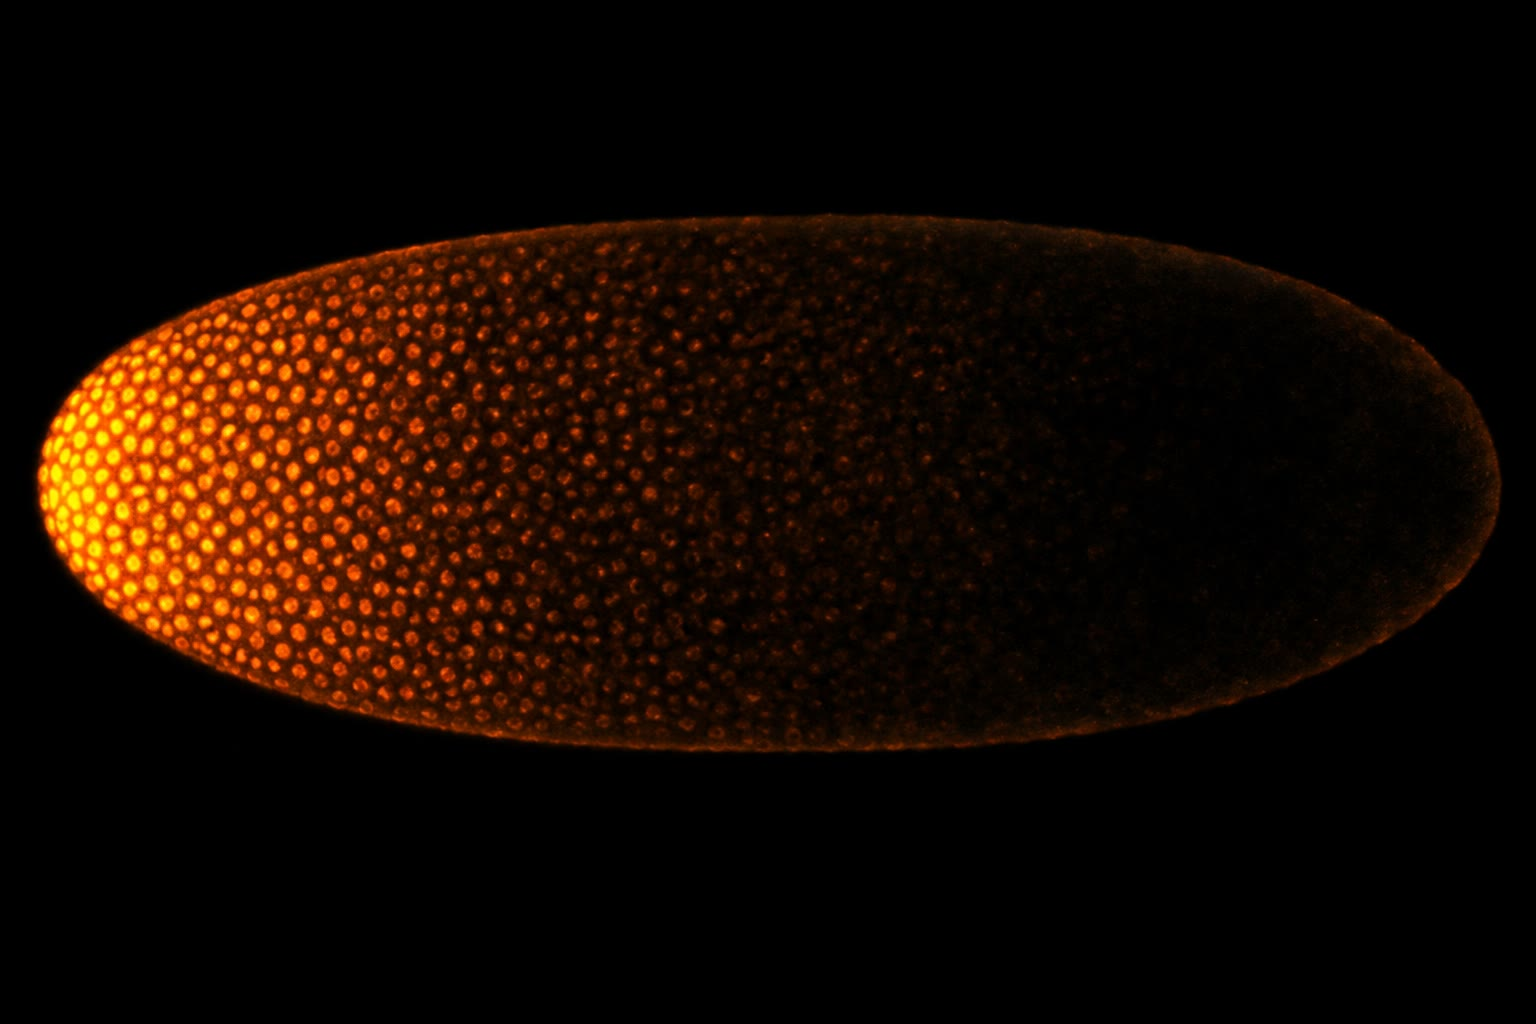
\includegraphics[width=0.46\linewidth]{images/book5/ai/b5-23-bicoid-gradient.jpg}\hspace{0.04\linewidth}
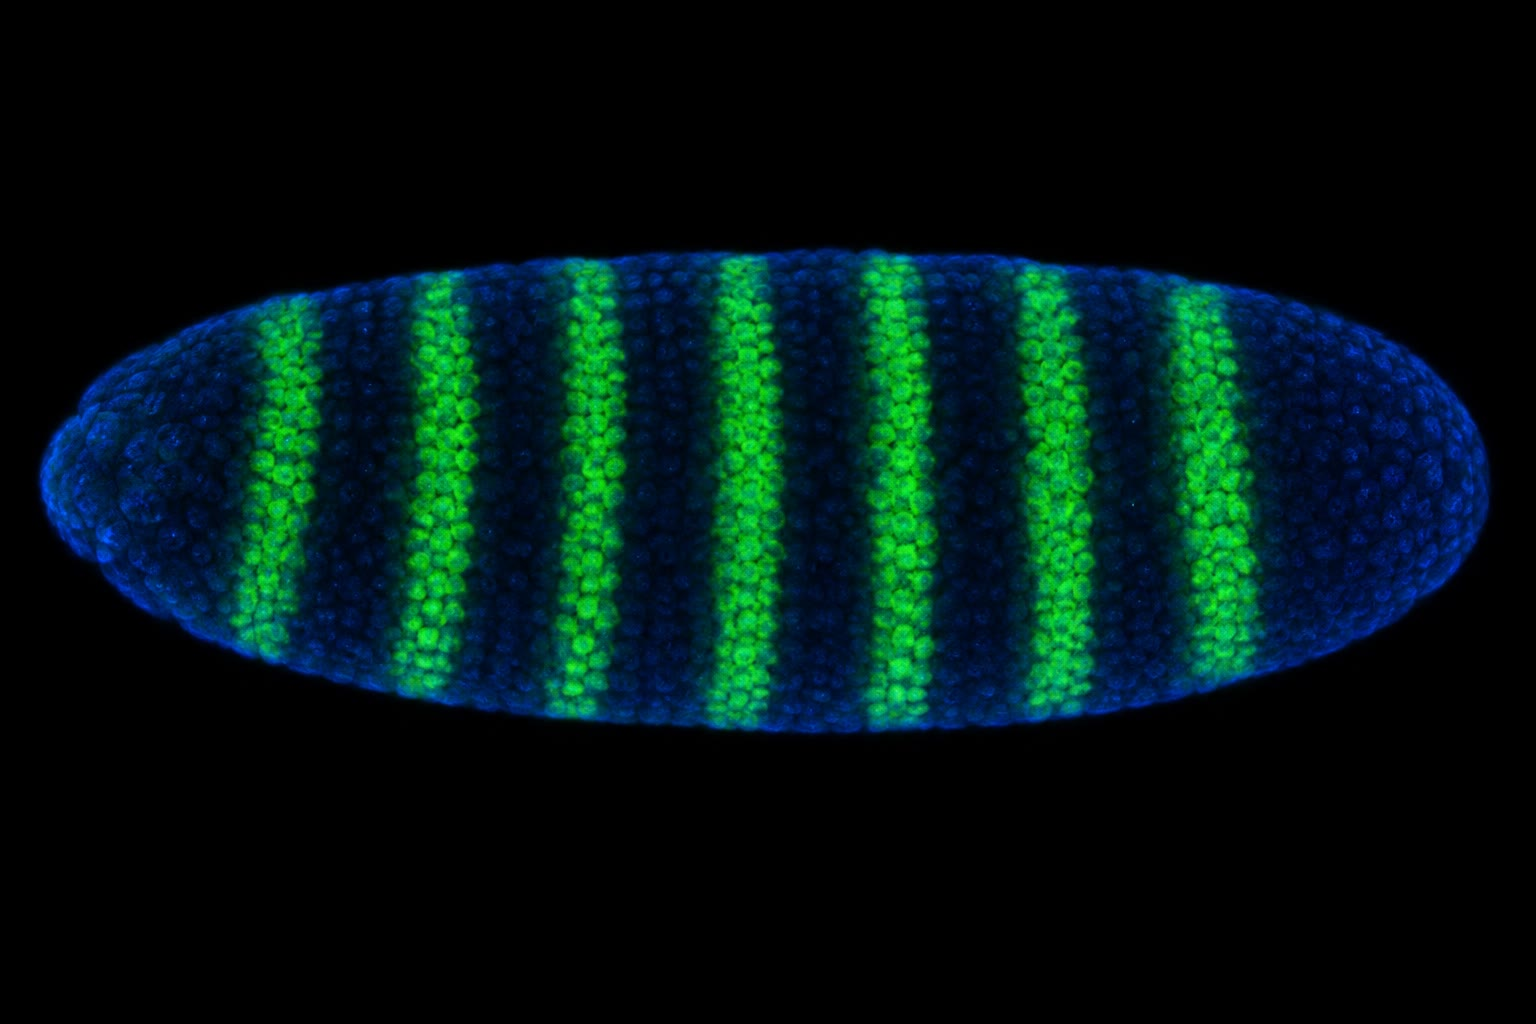
\includegraphics[width=0.46\linewidth]{images/book5/ai/b5-23-embryo-stripes.jpg}

{\small Kiri: sebuah embrio sinsitium yang diwarnai bagi protein Bicoid, paling terang
pada kutub depannya lalu memudar secara eksponensial ke arah belakangnya.
Kanan: sebuah embrio sejam kemudian yang diwarnai bagi sebuah protein aturan pasangan, tujuh
jalur yang digambar dari pita \omterm{def:b3:developmental-genetics:hierarchy}{gen senjangnya}.}
\end{omfigure}

\section{Jati diri: gen Hox}

\begin{definition}[Gen homeotik dan kolinearitas]\label{def:b3:developmental-genetics:hox}
\index{mutasi homeotik}\index{gen Hox}\index{kolinearitas}%
\index{homeobox}\index{sandi Hox}
Sebuah mutasi \emph{homeotik} mengubah satu bagian tubuh menjadi bagian lain:
itulah kata Bateson (1894) bagi kelainan yang ``menyulih satu
anggota sebuah deret dengan anggota lain.'' Pada lalatnya, mutan dominan
\emph{Antennapedia} menumbuhkan kaki di tempat sungutnya seharusnya; mutan
\emph{bithorax} (Lewis, 1978) mengubah segmen toraks ketiganya menjadi sebuah salinan
yang kedua, sehingga penyeimbangnya (halter) menjadi sepasang sayap yang
kedua. Kedelapan gen yang bertanggung jawab, yakni \emph{gen Hox}, terletak dalam dua
gugusan pada satu kromosom, dan Lewis memperhatikan bahwa urutannya sepanjang
DNA-nya memadani urutan sepanjang tubuh segmen yang dikendalikannya
--- itulah \emph{kolinearitas}, yang masih belum sepenuhnya terjelaskan. Masing-masing menyandi sebuah
faktor transkripsi dengan \omterm{def:b3:structural-biology:levels}{domain} pengikat DNA \emph{homeobox} beranggota
60 asam amino yang sama (McGinnis, Gehring, 1984), yang lalu ditemukan
pada tiap hewan: mencit dan manusia mengusung empat gugusan berisi tiga belas gen
masing-masing, yang kolinear dengan cara yang sama, yang diungkapkan dalam ranah bersarang sepanjang
sumbu tubuhnya, dengan gen yang lebih belakang pada gugusannya lebih ke belakang. Jati diri sebuah sel
sepanjang sumbunya diberikan oleh gabungan gen Hox yang
diungkapkannya, yakni \emph{sandi Hox}; gen belakangnya menguasai gen depannya
(keunggulan belakang), sehingga kehilangan sebuah gen belakang membuat segmennya
mengambil jati diri segmen di depannya. Gen Hox tidak membangun sebuah
segmen; mereka memberi tahu sebuah segmen yang sudah terbangun ia yang mana, dengan
menyalakan baterai gen hilir yang cocok bagi sebuah kaki, sebuah
sayap, sebuah rusuk, atau sebuah ruas tulang belakang pinggang.
\end{definition}

\begin{omfigure}
\begin{tikzpicture}[every node/.style={font=\scriptsize}, >=stealth]
  % fly cluster
  \node[left] at (-0.3,2.2) {lalat (\emph{Drosophila}), 8 gen};
  \foreach \i/\g/\c in {0/lab/omDef, 1/pb/omDef, 2/Dfd/omThm, 3/Scr/omThm, 4/Antp/omMeth, 5/Ubx/omMeth, 6/abd-A/omProp, 7/Abd-B/omProp} {
    \draw[thick, fill=\c!40] ({\i*1.1},1.9) rectangle ({\i*1.1+0.9},2.5); \node[font=\tiny] at ({\i*1.1+0.45},2.2) {\emph{\g}};
  }
  \node[left] at (-0.3,0.9) {gugusan HoxB mencit, 9 dari 13};
  \foreach \i/\g/\c in {0/b1/omDef, 1/b2/omDef, 2/b3/omDef, 3/b4/omThm, 4/b5/omThm, 5/b6/omMeth, 6/b7/omMeth, 7/b8/omProp, 8/b9/omProp} {
    \draw[thick, fill=\c!40] ({\i*1.1},0.6) rectangle ({\i*1.1+0.9},1.2); \node[font=\tiny] at ({\i*1.1+0.45},0.9) {\emph{\g}};
  }
  \draw[->, thick] (0,1.55) -- (9.8,1.55); \node[above, font=\tiny] at (4.9,2.55) {3$'$ $\to$ 5$'$ sepanjang DNA-nya};
  \draw[->, thick] (0,0.2) -- (9.8,0.2); \node[below, font=\tiny] at (4.9,0.05) {depan $\to$ belakang sepanjang tubuhnya};
  % body schematic
  \node[left] at (-0.3,-0.9) {diungkapkan di};
  \draw[thick, gray!70, rounded corners=6pt] (0,-1.3) rectangle (9.8,-0.5);
  \foreach \x/\t in {0.6/kepala, 2.6/leher, 4.4/toraks, 6.6/pinggang, 8.6/{sakrum, ekor}} { \node[font=\tiny] at (\x,-0.9) {\t}; }
  \draw[gray!70] (1.6,-1.3) -- (1.6,-0.5); \draw[gray!70] (3.5,-1.3) -- (3.5,-0.5); \draw[gray!70] (5.6,-1.3) -- (5.6,-0.5); \draw[gray!70] (7.6,-1.3) -- (7.6,-0.5);
  \node[below, align=center, font=\tiny] at (4.9,-1.4) {kolinearitas: urutan gennya pada kromosomnya adalah urutan ranahnya sepanjang tubuhnya;\\gugusan yang sama, urutan yang sama, dari lalat sampai mencit ---\\diwarisi dari sebuah nenek moyang 600 juta tahun lalu};
\end{tikzpicture}

{\small Gugusan Hox pada seekor lalat dan seekor mencit. Gennya terletak sepanjang DNA-nya dalam
urutan daerah tubuh yang ditentukannya, pada kedua hewannya, dan gen
homolognya dapat dikenali lewat urutannya: sebuah gen \emph{Hoxb6} mencit
dapat dikenali sebagai \emph{Antennapedia} milik lalatnya.}
\end{omfigure}

\begin{proof}[Bukti eksperimental]
Lewis (1978) memetakan kompleks \emph{bithorax} sebagai sebuah deret
mutasi yang masing-masing mengubah satu segmen menjadi segmen di depannya, yang tersusun
pada kromosomnya dalam urutan tubuhnya, lalu mengusulkan bahwa gennya
diaktifkan berurutan sepanjang sumbunya. McGinnis dan rekannya (1984)
menemukan \omterm{def:b3:developmental-genetics:hox}{homeoboxnya} lewat hibridisasi silang antara \emph{Antennapedia}
dan \emph{Ultrabithorax} lalu pada katak dan mencit. Kesetaraan fungsinya
ditunjukkan langsung: sebuah gen \emph{Hoxb6} mencit yang diungkapkan pada seekor
lalat menghasilkan fenotipe \emph{Antennapedia}, yakni kaki dari sungut
(dasawarsa 1990-an); seekor mencit tanpa \emph{Hoxc8} punya sebuah rusuk tambahan pada ruas
tulang belakang pinggang pertamanya, dengan segmennya mengambil jati diri segmen di
depannya; dan mengubah batas pengungkapan Hox pada ayam dan mencit menggeser
kedudukan tempat anggota depannya terbentuk, dengan panjang leher seekor angsa
dipadani sebuah geseran ke belakang batas yang sama.
\end{proof}

\begin{omfigure}
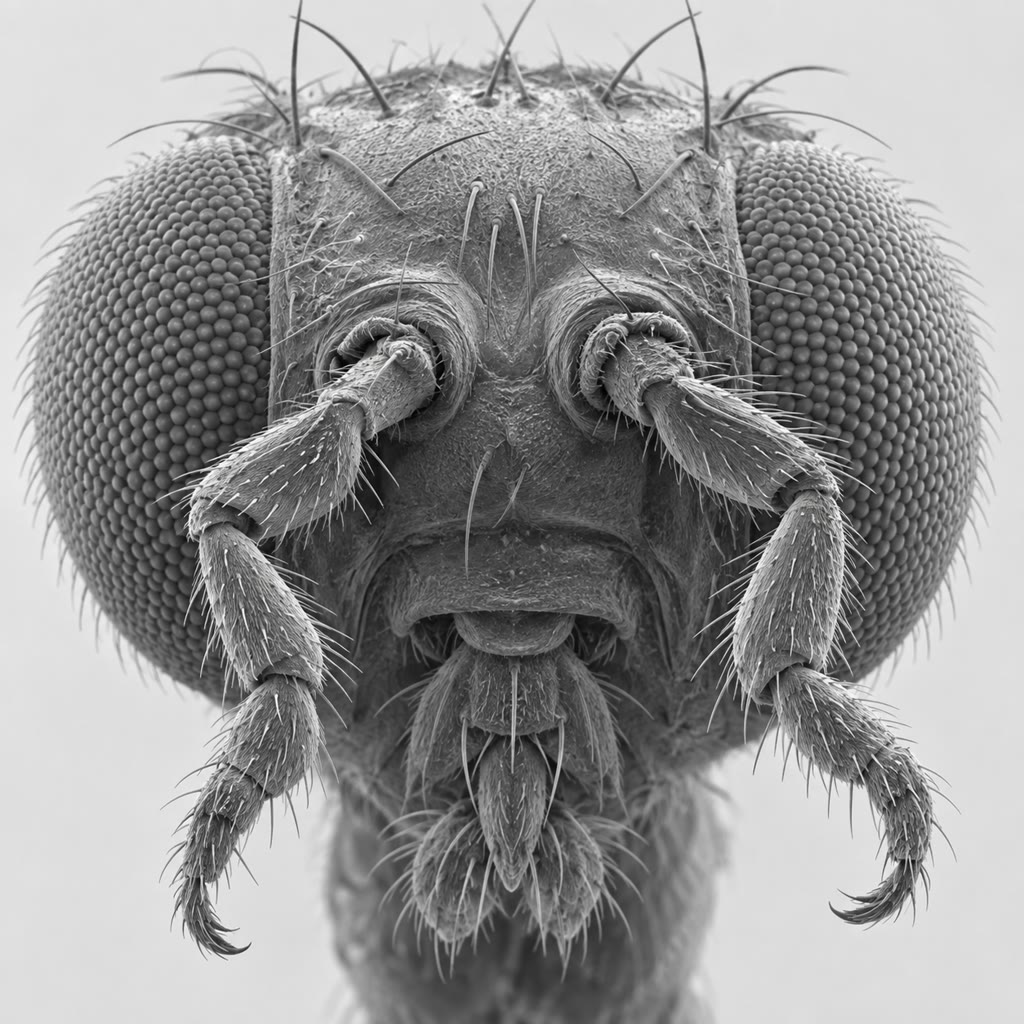
\includegraphics[width=0.34\linewidth]{images/book5/ai/b5-23-antennapedia-fly.jpg}\hspace{0.04\linewidth}
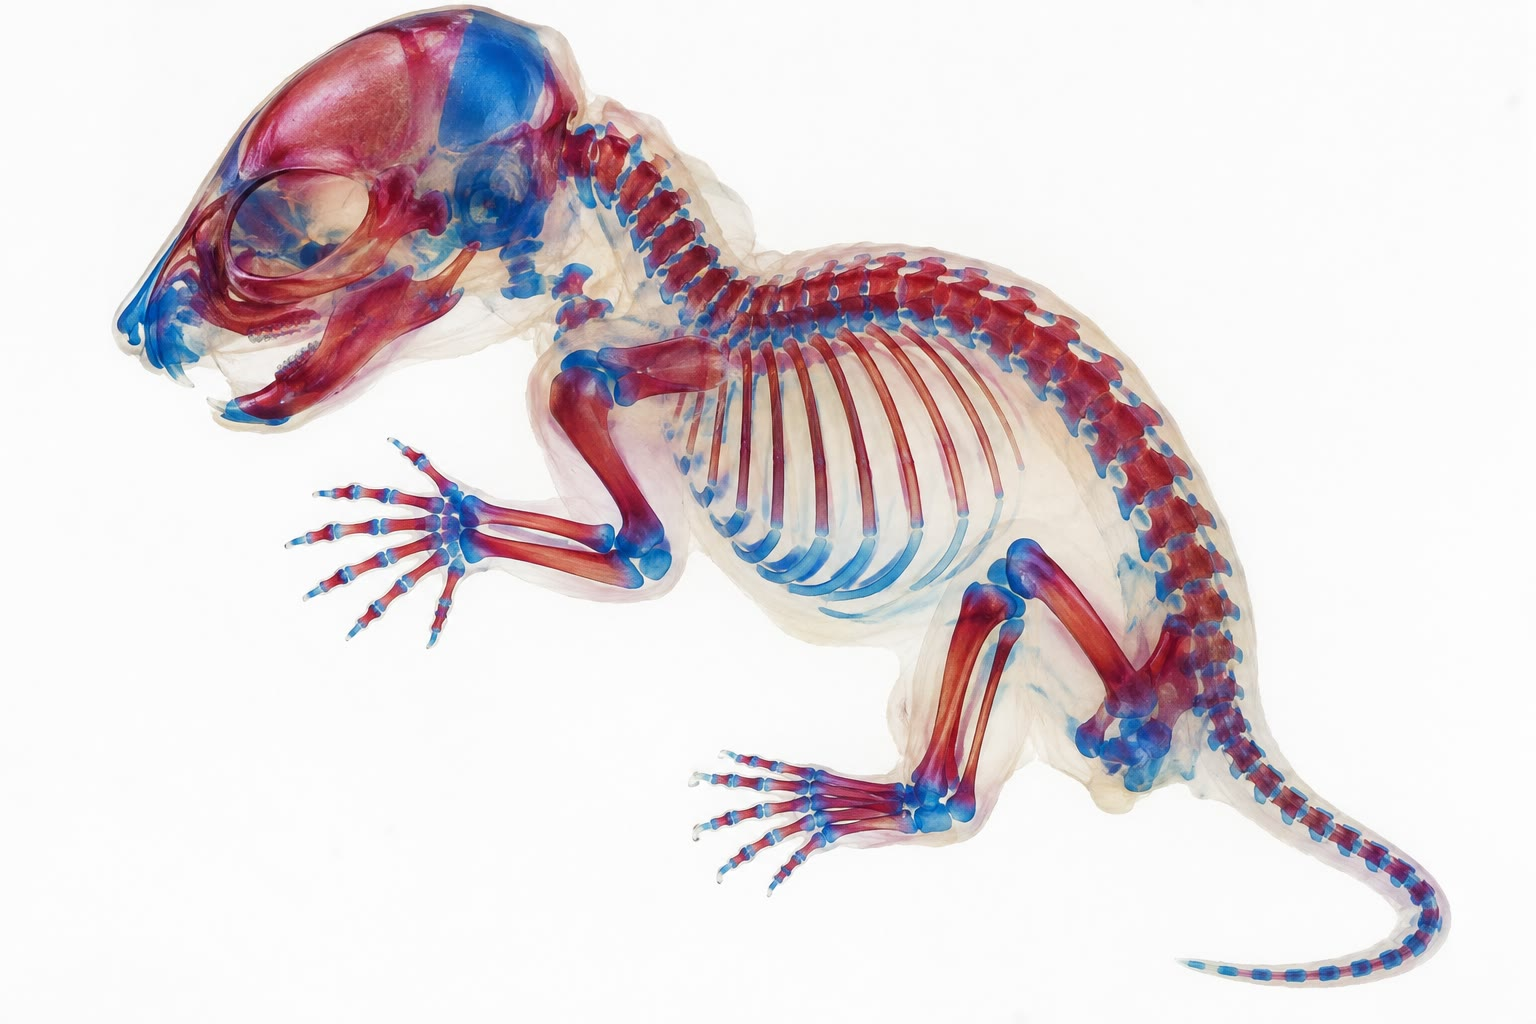
\includegraphics[width=0.5\linewidth]{images/book5/ai/b5-23-limb-skeleton-stain.jpg}

{\small Kiri: kepala seekor lalat mutan \emph{Antennapedia}, sepasang
kaki di tempat sungutnya seharusnya --- segmennya terbangun dengan benar lalu
diberi tahu jati diri yang salah. Kanan: rangka sebuah embrio mencit, dengan tulang rawannya
biru dan tulangnya merah, yakni ruas tulang belakang yang sepanjangnya \omterm{def:b3:developmental-genetics:hox}{sandi Hox} dibaca.}
\end{omfigure}

\section{Membangun seekor vertebrata}

\begin{definition}[Penata dan pusat pengisyaratan]\label{def:b3:developmental-genetics:organiser}
\index{penata}\index{pengimbasan}\index{sonic hedgehog}\index{tunas anggota badan}%
\index{zona keaktifan pengutuban}\index{rabung ektoderma apikal}
Embrio vertebrata bersel sejak awalnya, sehingga landaiannya
dibuat protein yang disekresikan alih-alih pembauran sebuah sinsitium, dan
beberapa keluarga yang sama mengerjakan segalanya: Wnt, Hedgehog, BMP dan kerabat
TGF-$\beta$ lain, FGF, Notch, serta asam retinoat. Spemann dan Mangold (1924)
mencangkokkan sepotong bibir punggung sebuah gastrula kadal air ke perut
kadal air lain lalu memperoleh sebuah embrio kedua, dari kepala sampai ekor, yang terbuat kebanyakan dari
sel inangnya: cangkoknya adalah sebuah \emph{penata}, yang mengimbas tetangganya untuk
membentuk sebuah sistem saraf dan sumbu, dan molekulnya ditemukan tujuh puluh
tahun kemudian berupa penentang yang disekresikan (Chordin, Noggin) yang menghalangi
BMP, yang ketiadaannya membuat ektodermanya menjadi saraf --- yakni keadaan bawaannya.
\emph{Tabung sarafnya} lalu dipola dari punggung ke perut oleh \emph{sonic
hedgehog} dari notokorda dan pelat lantainya (tinggi: neuron motorik; rendah:
\omterm{def:b3:nervous-systems:cells}{interneuron}) melawan BMP dari atapnya; dan \emph{tunas anggota badannya} oleh dua
pusat, yakni \emph{zona keaktifan pengutuban} pada tepi belakangnya
yang menyekresikan Shh (cangkoknya ke tepi depannya memberi sebuah penggandaan
cermin jari-jarinya, yakni enam jari yang bertemu ibu jari lawan ibu jari) dan
\emph{rabung ektoderma apikal} pada pucuknya yang menyekresikan FGF yang menjaga
sel di bawahnya tetap membelah lalu menentukan urutan dari dekat ke jauh
tulang lengan atas, lengan bawah, dan tangannya. Pencangkokan, pembuangan, dan manik yang direndam
protein tetap menjadi perkakasnya; logikanya --- sebuah sumber setempat, sebuah landaian,
ambang, sebuah sandi faktor transkripsi --- adalah logika lalatnya.
\end{definition}

\begin{omfigure}
\begin{tikzpicture}[every node/.style={font=\scriptsize}, >=stealth]
  % limb bud
  \fill[omDef!12] (0,0) -- (0,3) .. controls (2.6,3.4) and (3.4,2.2) .. (3.4,1.5) .. controls (3.4,0.8) and (2.6,-0.4) .. (0,0) -- cycle;
  \draw[thick, omDef] (0,0) -- (0,3) .. controls (2.6,3.4) and (3.4,2.2) .. (3.4,1.5) .. controls (3.4,0.8) and (2.6,-0.4) .. (0,0);
  \draw[very thick, omMeth!70!black] (2.9,2.5) .. controls (3.45,1.9) and (3.45,1.1) .. (2.9,0.5);
  \node[right, align=left, omMeth!70!black, font=\tiny] at (3.5,1.5) {rabung ektoderma apikal:\\FGF8; menjaga\\zona kemajuannya tetap membelah;\\dekat $\to$ jauh};
  \begin{scope}
    \clip (0,0) -- (0,3) .. controls (2.6,3.4) and (3.4,2.2) .. (3.4,1.5) .. controls (3.4,0.8) and (2.6,-0.4) .. (0,0) -- cycle;
    \foreach \i/\op in {1/50, 2/38, 3/26, 4/14} { \draw[omThm!\op, thick] (0.6,0.5) circle ({0.45*\i}); }
  \end{scope}
  \fill[omThm!50] (0.6,0.5) ellipse (0.5 and 0.35); \node[anchor=north, align=center, omThm, font=\tiny] at (0.9,-0.2) {ZPA: sonic hedgehog,\\belakang $\to$ depan};
  \node[left, font=\tiny] at (-0.05,2.6) {depan}; \node[left, font=\tiny] at (-0.05,0.4) {belakang};
  \node[left, font=\tiny] at (-0.05,1.5) {dinding tubuh};
  \draw[->, thick] (0.3,1.5) -- (3.0,1.5); \node[above, font=\tiny] at (1.75,1.55) {lengan atas, lengan bawah, jari};
  % right: digit code
  \node[right, align=left] at (7.2,2.6) {jati diri jari dari pemaparan Shh:\\ibu jari (jari 1): tanpa Shh;\\jari 2--3: landaian;\\jari 4--5: dari sel pengungkap Shh};
  \node[right, align=left] at (7.2,1.0) {cangkokkanlah sebuah ZPA kedua di depan:\\penggandaan cermin, 4-3-2-2-3-4;\\manik protein Shh melakukan hal yang sama};
  \node[right, align=left, gray] at (7.2,-0.2) {molekul yang sama memola tabung sarafnya\\(neuron motorik tempat ia tinggi) dan ususnya};
\end{tikzpicture}

{\small Kedua pusat pengisyaratan \omterm{def:b3:developmental-genetics:organiser}{tunas anggota badannya}. \omterm{def:b3:developmental-genetics:organiser}{Sonic hedgehog} dari
tepi belakangnya memberi tahu selnya harus menjadi jari yang mana; FGF dari pucuknya
memberi tahu seberapa jauh mereka sepanjang anggota badannya. Cangkok yang memindahkan sebuah
pusat memindahkan polanya bersamanya.}
\end{omfigure}

\begin{proposition}[Pola yang timbul sendiri: mekanisme Turing]\label{prop:b3:developmental-genetics:turing}
\index{pola Turing}\index{reaksi--pembauran}\index{pengaktif--penghambat}
Tidak setiap pola dibaca dari sebuah landaian yang sudah ada. Turing (1952)
menunjukkan bahwa dua zat yang membaur yang bereaksi --- sebuah \emph{pengaktif}
yang merangsang produksinya sendiri dan produksi sebuah \emph{penghambat},
dan sebuah penghambat yang menekan pengaktifnya lalu membaur jauh
lebih cepat --- dapat mengubah sebuah medan yang seragam menjadi sebuah larik puncak yang teratur
dengan sendirinya: sebuah kelebihan pengaktif setempat yang kecil tumbuh lewat
peningkatan diri sementara penghambat yang dihasilkannya menyebar keluar lalu
mencegah puncak baru terbentuk di dekatnya, sehingga puncaknya muncul pada sebuah jarak yang ditetapkan
jangkauan penghambatnya, $\lambda \sim \sqrt{D_{\text{inh}}/k_{\text{inh}}}$,
dan bukan oleh koordinat luar mana pun. Mekanismenya, yang matematikanya
diakui saja di sini, adalah keterangan terbaik bagi bintik dan jalur mantel
hewan, jarak folikel rambut dan tunas bulunya, rabung
langit-langitnya, jari tangannya (yang cacahnya naik ketika
panjang gelombang polanya dipendekkan dengan menurunkan keaktifan Hox), serta
jalur ikan zebra, yang selnya yang saling berinteraksi --- yakni sel pigmen
yang menolak tetangga dari satu jenis lalu menarik tetangga dari jenis lain pada sebuah
jarak --- telah dikenali dan jalurnya dibuat terbentuk ulang
sesudah pembuangan laser tepat seperti yang diramalkan teorinya.
\end{proposition}
\admitted

\section{Evolusi bentuk}

\begin{definition}[Evo-devo: perkakas dan sakelar]\label{def:b3:developmental-genetics:evodevo}
\index{homologi dalam}\index{perkakas genetik}%
\index{evolusi pengatur-sis}\index{heterokroni}
Gen yang membangun hewan adalah sebuah \emph{perkakas} yang purba dan dipakai bersama:
beberapa ratus faktor transkripsi dan jalur pengisyaratan yang hadir
pada nenek moyang bersama semua hewan, dan keanekaan hewan datang
kebanyakan dari perubahan pada \emph{kapan, di mana, dan seberapa banyak} gen itu
diungkapkan alih-alih pada apa yang disandinya. \emph{Homologi dalam}: gen
\emph{Pax6} mengarahkan pembentukan mata pada lalat, cumi-cumi, dan mencit, yang
matanya tidak homolog sebagai organ --- sebuah \emph{Pax6} mencit yang diungkapkan pada
kaki seekor lalat membuat sebuah mata lalat yang salah tempat di sana (Halder, Gehring, 1995).
\emph{Evolusi pengatur-sis}: hilangnya duri panggul pada
ikan duri air tawar adalah penghapusan satu penggalak gen
\emph{Pitx1}, dengan proteinnya tak tersentuh dan masih melayani di tempat lain;
hilangnya bintik sayap pada sebagian lalat buah adalah sebuah perubahan pada sebuah penggalak
\emph{yellow}; hilangnya kaki pada ular adalah sebuah penggalak
\emph{\omterm{def:b3:developmental-genetics:organiser}{sonic hedgehog}} yang rusak pada anggota badannya. \emph{Geseran Hox}: batas
pengungkapan \emph{Hoxc6} menandai ruas tulang belakang toraks pertama pada mencit,
ayam, angsa, dan ular sama saja, pada ruas 7, 14, 23, dan 3; hilangnya
kaki perut pada serangga adalah protein Hox Ubx yang memperoleh sebuah ranah penekan
yang mematikan gen kaki \emph{Distal-less}, yang pada krustasea ia tidak
melakukannya. \emph{Heterokroni}, yakni sebuah perubahan pada waktu sebuah
acara perkembangan, menjadikan aksolotl sebuah larva yang tetap dan wajah
manusia wajah sebuah kera muda. Pertanyaan lama tentang bagaimana bentuk baru timbul
menjadi sebuah pertanyaan tentang DNA pengatur: kebanyakan genom yang
berarti bagi bentuknya bukanlah gen melainkan sakelar.
\end{definition}

\begin{example}[Empat sayap]\label{ex:b3:developmental-genetics:four-wings}
Nenek moyang lalat punya empat sayap, seperti masih dipunyai capung dan lebah;
lalat punya dua, dengan pasangan belakangnya menyusut menjadi penyeimbangnya. Pada lalat,
\emph{Ultrabithorax} diungkapkan pada segmen toraks ketiganya lalu
menekan acara sayapnya di sana --- sekitar seratus gen sasaran, dengan sebuah
halter berupa sebuah sayap dengan gen itu dimatikan. Lalat mutan rangkap tiga milik Lewis,
yang tidak punya fungsi \emph{Ubx} pada segmen ketiganya,
menumbuhkan sepasang sayap kedua: bukan sebuah struktur baru melainkan pelepasan
sebuah struktur lama. Pada kupu-kupu, \emph{Ubx} diungkapkan pada sayap belakangnya pula,
dan di sana ia tidak menekan sayapnya melainkan mengubah polanya:
protein yang sama, sehimpunan sasaran yang berbeda. Empat ratus juta
tahun evolusi diptera berporos pada keputusan satu gen pada satu
segmen, dan sebuah mutasi tunggal membatalkannya dalam satu angkatan --- dan itulah
sebabnya sejarah bentuknya terbaca pada gen yang membangunnya.
\end{example}

\begin{remark}[Geometri dari kimia]\label{rem:b3:developmental-genetics:remark}
Sebuah embrio tidak punya cetak biru dan tidak punya juru ukur. Ia punya beberapa landaian
yang dibuat lewat pembauran dan peluruhan, sel yang membacanya terhadap ambang
lalu menyalakan faktor transkripsi, serta sebuah sandi faktor itu yang
memberi tahu tiap daerahnya harus menjadi apa; ia punya \omterm{def:b3:developmental-genetics:organiser}{penata} setempat yang mengimbas
tetangganya, dan reaksi yang memola dirinya sendiri. Matematikanya
adalah matematika kinetika orde satu dan pembauran --- sebuah
eksponensial, sebuah akar kuadrat, sebuah ambang --- dan ia menjelaskan bukan hanya
bagaimana kepala seekor lalat ditaruh melainkan mengapa melipatduakan sebuah gen menggeser sebuah batas
sejauh yang tetap, mengapa enam jari muncul ketika sebuah isyarat
digandakan, dan mengapa seekor ular punya tiga ratus rusuk. Evolusi menyunting
sakelarnya, bukan mesinnya: perkakas sebuah bunga karang dan seorang manusia
nyaris sama, dan yang berbeda adalah perangkaiannya.
\end{remark}

\section{Latihan}

\begin{exercise}[$\star$]\label{exo:b3:developmental-genetics:1}
Namailah keempat tingkat hierarki segmentasi lalatnya, satu gen tiap
tingkatnya, dan fenotipe mutan yang menaruhnya di kelasnya.
\end{exercise}

\begin{exercise}[$\star$]\label{exo:b3:developmental-genetics:2}
Apa itu sebuah \omterm{def:b3:developmental-genetics:hierarchy}{gen pengaruh induk}? Seekor betina yang homozigot bagi sebuah mutasi
nol \emph{bicoid} dikawinkan dengan seekor jantan liar: perikanlah embrionya lalu
jelaskanlah mengapa genotipenya sendiri tidak menyelamatkannya.
\end{exercise}

\begin{exercise}[$\star$]\label{exo:b3:developmental-genetics:3}
Nyatakanlah \omterm{def:b3:developmental-genetics:hox}{kolinearitas} dan keunggulan belakang. Ramalkanlah fenotipe seekor
mencit tanpa \emph{Hoxc8} dan seekor lalat yang mengungkapkan \emph{Antennapedia}
di kepalanya.
\end{exercise}

\begin{exercise}[$\star$]\label{exo:b3:developmental-genetics:4}
Apa yang ditunjukkan cangkok Spemann--Mangold, dan ternyata apa molekul
\omterm{def:b3:developmental-genetics:organiser}{penatanya}? Mengapa nasib saraf disebut ``bawaan''?
\end{exercise}

\begin{exercise}[$\star\star$]\label{exo:b3:developmental-genetics:5}
Bicoid: $D = \qty{4}{\micro m^2/s}$, paruh hidup \qty{35}{min}. Hitunglah
$k$, $\lambda$, dan nisbah kepekatan pada kutub depannya dan
di tengah telurnya (\qty{250}{\micro m}).
\end{exercise}

\begin{exercise}[$\star\star$]\label{exo:b3:developmental-genetics:6}
Dengan $\lambda = \qty{100}{\micro m}$, sebuah batas duduk pada
\qty{240}{\micro m}. Di mana ia duduk bila induknya mengusung empat salinan
\emph{bicoid} alih-alih dua? Satu salinan? Nyatakanlah geserannya sebagai sebuah
pecahan sebuah telur \qty{500}{\micro m}.
\end{exercise}

\begin{exercise}[$\star\star$]\label{exo:b3:developmental-genetics:7}
Inti pada blastodermanya berjarak \qty{8}{\micro m}. Untuk menaruh sebuah
batas sampai dalam satu inti dengan $\lambda = \qty{100}{\micro m}$,
seberapa cermat sebuah inti harus membaca kepekatan Bicoidnya? Bila
intinya mencacah molekul sepanjang sebuah waktu $\tau$ dan cacahnya Poisson,
berapa banyak yang harus dicacahnya?
\end{exercise}

\begin{exercise}[$\star\star$]\label{exo:b3:developmental-genetics:8}
Landaiannya mendekati keadaan mantap pada skala waktu $1/k$. Dengan sebuah
paruh hidup \qty{35}{min}, berapa pecahan kepekatan keadaan mantapnya
yang tercapai pada \qty{60}{min}, \qty{90}{min}, dan
\qty{120}{min}? Apa yang disiratkannya bagi sebuah embrio yang harus membaca
landaiannya pada \qty{150}{min}?
\end{exercise}

\begin{exercise}[$\star\star$]\label{exo:b3:developmental-genetics:9}
Sebuah ZPA dicangkokkan ke tepi depan sebuah \omterm{def:b3:developmental-genetics:organiser}{tunas anggota badan} ayam. Ramalkanlah
pola jarinya, dan polanya bila justru sebuah manik yang melepaskan dosis rendah
Shh ditanamkan di sana.
\end{exercise}

\begin{exercise}[$\star\star\star$]\label{exo:b3:developmental-genetics:10}
Sebuah morfogen dibuat di seluruh sebuah jaringan sepanjang $L$ pada laju $s$ tiap
satuan volume, dirombak pada laju $k$, lalu dimusnahkan pada batas $x =
L$ (sebuah sumur penyerap), tanpa fluks pada $x = 0$. Selesaikanlah $Dc'' - kc + s =
0$ bagi $c(x)$ lalu sketsalah. Bagaimana bentuk landaian ini berbeda dari
hal sumber-pada-satu-ujungnya, dan apa yang terjadi ketika $L \ll \lambda$?
\end{exercise}

\begin{exercise}[$\star\star\star$]\label{exo:b3:developmental-genetics:11}
Dua ambang pada $T_{1} = 0.3c_{0}$ dan $T_{2} = 0.08c_{0}$ membagi sebuah
landaian menjadi tiga daerah. Tunjukkanlah bahwa lebar kedua daerah pertamanya
tidak bergantung pada $c_{0}$, lalu jelaskanlah mengapa sebuah embrio yang
\emph{panjangnya} beragam antarindividu (\qty{450}{} sampai
\qty{550}{\micro m}) memerlukan sesuatu yang lebih daripada sebuah eksponensial tunggal untuk
menskalakan polanya. Usulkanlah satu mekanisme.
\end{exercise}

\begin{exercise}[$\star\star\star$]\label{exo:b3:developmental-genetics:12}
Ikan duri kehilangan duri panggulnya dengan menghapus sebuah penggalak \emph{Pitx1},
ular kehilangan anggota badannya dengan merusak sebuah penggalak \emph{\omterm{def:b3:developmental-genetics:organiser}{sonic hedgehog}}. Jelaskanlah
mengapa perubahan pengatur alih-alih perubahan penyandi yang menjadi jalan lazim
menuju sebuah struktur yang hilang atau berubah, menurut pleiotropi dan menurut apa yang
dikerjakan protein yang sama di tempat lain.
\end{exercise}

\section{Soal: Bendera Prancis}

\begin{problem}[{Soal akhir pekan --- sistem koordinat sebuah telur yang dihitung
dari kinetika orde satu: panjang landaian Bicoidnya, sumbernya dan waktu
pembentukannya, batas yang digambarnya dan kecermatannya, apa yang dilakukan dosis gen
dan ukuran telurnya terhadapnya, serta sandi Hox yang dibaca di hilirnya, berakhir pada
panjang peluruhannya, geseran tiap penggandaannya, dan kecermatan kedudukannya}]
\label{pb:b3:developmental-genetics:1}
Data: panjang telur \qty{500}{\micro m}; Bicoid $D = \qty{4}{\micro m^2/s}$,
paruh hidup \qty{35}{min}; fluks sumbernya sedemikian sehingga $c_{0} = \qty{50}{nM}$
dengan dua salinan induk; jarak inti \qty{8.5}{\micro m} pada daur
14; ambang $T_{1} = 0.3\,c_{0}$ (kepala/toraks) dan $T_{2} =
0.08\,c_{0}$ (batas \emph{hunchback}) bagi hal dua salinannya. Derau
pembacaan $\delta c/c = 0.1$ bagi sebuah inti tunggal. Bilangan Avogadro
\qty{6e23}{}; sebuah inti adalah sebuah bola berjejari \qty{3}{\micro m}.

\medskip
\noindent\textbf{Bagian I --- Landaiannya.}
\begin{enumerate}
  \item Hitunglah $k$ dari paruh hidupnya, dalam \unit{s^{-1}}, dan
        umurnya $1/k$ dalam menit.
  \item Hitunglah $\lambda = \sqrt{D/k}$ dalam mikrometer. Berapa \omterm{thm:b3:developmental-genetics:gradient}{panjang
        peluruhan} telurnya?
  \item Kepekatannya turun sebesar faktor berapa dari kutub ke kutub? Sebesar
        faktor berapa sepanjang satu jarak inti di tengah telurnya?
  \item Hitunglah fluks sumbernya $J = c_{0}\sqrt{Dk}$ dalam
        \unit{nM\,\micro m\,s^{-1}}, dan cacah molekul
        yang memasuki sepetak \qty{1}{\micro m^2} kutub depannya tiap
        detik.
  \item Berapa cacah molekul Bicoid di dalam sebuah inti pada kutubnya ($c_{0}$)
        dan di tengah telurnya?
  \item Berapa pecahan keadaan mantap yang tercapai pada \qty{60}{min} dan
        \qty{120}{min} ($1 - \mathrm{e}^{-kt}$)? Apakah landaiannya mantap
        ketika batasnya digambar, pada sekitar \qty{120}{min}?
\end{enumerate}

\medskip
\noindent\textbf{Bagian II --- Batasnya.}
\begin{enumerate}[resume]
  \item Kedudukan kedua batasnya, dalam \unit{\micro m} dan sebagai
        pecahan panjang telurnya.
  \item Induknya punya empat salinan: berapa $c_{0}$ barunya, dan berapa kedua kedudukan
        batasnya? Masing-masing bergerak sejauh berapa? Enam salinan?
  \item Satu salinan: berapa kedudukannya? Daerah mana yang tumbuh, mana yang menyusut?
  \item Berapa galat kedudukan dari sebuah derau pembacaan \qty{10}{\%}, dalam
        mikrometer dan dalam jarak inti?
  \item Bila galatnya harus satu inti, kecermatan pembacaan berapa yang
        diperlukan? Bila intinya merata-rata atas $n$ pembacaan yang bebas
        dan deraunya turun sebagai $1/\sqrt{n}$, berapa banyak pembacaannya?
  \item Sebuah inti pada batas \emph{hunchback}-nya memuat cacah
        yang dihitung pada pertanyaan~5. Berapa derau Poisson
        $1/\sqrt{N}$ sebuah cacahan seketika yang tunggal? Bandingkanlah dengan
        \qty{10}{\%} lalu berilah ulasan.
\end{enumerate}

\medskip
\noindent\textbf{Bagian III --- Penskalaan dan ketangguhan.}
\begin{enumerate}[resume]
  \item Telurnya beragam dari \qty{450}{} sampai \qty{550}{\micro m}. Bila $\lambda$
        dan $c_{0}$ terpancang, di mana batas \emph{hunchback}-nya
        jatuh sebagai sebuah pecahan panjang telurnya pada masing-masing? Apakah polanya terskala?
  \item Andaikanlah justru $D$ berskala sebagai $L^{2}$ (dengan umur yang sama,
        tetapi sebuah sumber yang sebarannya tumbuh bersama telurnya). Tunjukkanlah bahwa
        $\lambda/L$ lalu tetap dan polanya terskala. Masuk akalkah ini?
  \item Gen \emph{hunchback} menanggapi Bicoid dengan sebuah \omterm{def:b3:structural-biology:allostery}{koefisien
        Hill} $5$: pengungkapannya adalah $c^{5}/(c^{5} + T^{5})$.
        Sepanjang berapa mikrometer pengungkapannya beranjak dari \qty{10}{\%}
        ke \qty{90}{\%} di sekitar batasnya? Bandingkanlah dengan satu jarak inti.
  \item Jelaskanlah mengapa sebuah tanggapan yang curam menajamkan sebuah batas tetapi tidak
        dengan sendirinya memangkas galat kedudukan yang disebabkan derau
        kepekatannya.
  \item Penekanan timbal balik antara \omterm{def:b3:developmental-genetics:hierarchy}{gen senjang} menajamkan dan memantapkan
        batasnya. Berhujahlah dalam sebuah kalimat mengapa dua gen yang saling menekan
        tidak dapat kedua-duanya menyala di dalam inti yang sama pada keadaan
        mantap.
  \item Suhu menaikkan $D$ sebesar \qty{2}{\%} dan $k$ sebesar \qty{6}{\%} tiap
        derajat. Berapa perubahan $\lambda$ tiap derajat, dan berapa geseran batasnya
        bagi sebuah ruangan yang \qty{5}{\celsius} lebih hangat? Mengapa embrio mungkin memerlukan sebuah
        mekanisme pengimbang?
\end{enumerate}

\medskip
\noindent\textbf{Bagian IV --- Jati diri.}
\begin{enumerate}[resume]
  \item \omterm{def:b3:developmental-genetics:hox}{Sandi Hox}: dengan delapan \omterm{def:b3:developmental-genetics:hox}{gen Hox} lalat yang masing-masing menyala atau mati, berapa banyak
        sandi yang mungkin? Berapa banyak yang dipakai (empat belas segmen)? Mengapa
        keunggulan belakang memangkas cacah mujarabnya?
  \item Seekor lalat tidak punya \emph{Ubx} pada segmen toraks ketiganya. Segmennya
        menjadi apa, dan mengapa hasilnya empat sayap dan bukan sebuah
        struktur baru?
  \item Batas \emph{Hoxc6} seekor mencit terletak pada ruas tulang belakang 7, milik seekor angsa pada
        23. Apa yang diramalkannya tentang lehernya, dan apa yang berubah
        pada evolusinya: gennya, atau pengungkapannya?
  \item Sebuah cangkok ZPA memberi jari 4-3-2-2-3-4. Jelaskanlah polanya dari
        dua landaian Shh yang bertemu di tengahnya.
  \item Halder dan Gehring mengungkapkan \emph{Pax6} mencit pada kaki seekor lalat
        lalu memperoleh sebuah mata lalat di sana. Apa yang ditunjukkannya tentang
        gennya, dan apa yang \emph{tidak} ditunjukkannya tentang mata lalat
        dan mencit?
  \item Jari keenam: memendekkan panjang gelombang Turing menambahkan sebuah jari.
        Dengan lima jari melintasi sebuah lempeng tangan \qty{2}{mm}, perubahan panjang
        gelombang berapa yang memberi enam? Parameter mana dari sistem
        reaksi--pembaurannya yang akan menghasilkannya?
  \item Ringkaslah: $\lambda$ (pertanyaan~2), geseran batas tiap
        penggandaan sumbernya (pertanyaan~8), dan galat kedudukan
        dari derau \qty{10}{\%} (pertanyaan~10).
\end{enumerate}
\end{problem}
